\section{第4問：小町算の探索と高精度な$\sqrt{2}$近似}
\label{sec:q04}

\subsection{探索目標と有限な文法}
数字$1,2,\ldots,9$を各1回、順番通りに用いる条件で、式$e$の値$v(e)$を$\sqrt{2}$へ近づけた。
探索法そのものの比較と、精度を追求する追加探索を実施した。
課題ページの$\sqrt{2}$の表示には誤植があるため、正しい値
$1.414213562373095\ldots$を基準にする。
元の式を有理数で再計算すると、順序固定の例は$6883/4867$で、絶対誤差は$4.6418595\times10^{-6}$である。
並べ替え例のうち最初の式も、実際には$390050/275807=1.41421356238239\ldots$となる。
元の数式と表示された近似小数を区別して検証した。

式の文法を明示しないと、階乗の繰り返しなどで探索空間が際限なく増える。
本実験では、葉を「連続する数字の連結整数」「その連結に小数点を1個入れた値」「1桁の数字の階乗」のいずれかとし、内部節点を四則演算とした。
複合式全体の階乗は含めない。
ゼロ除算を除外し、途中値の絶対値を$10^9$以下、既約分母を80 bit以下に制限した。
以下の完全性・最短性は、この有限な文法内での性質である。
小数は例えば$.12=3/25$として扱い、状態のキーには浮動小数点数を使わない。

\subsection{同じ状態グラフでDFS・BFS・A*を比較する}
逆ポーランド記法の状態を
\[
 s=(i;v_1,\ldots,v_k)
\]
と定義した。$i$は使用済み数字数、後半は有理数のスタックである。
未使用の連続数字から葉を1個積む操作と、上位2値を四則演算で1値にまとめる操作を生成する。
全数字を消費してスタックが1個となり、
$|v_1-\sqrt{2}|\leq\varepsilon$を満たせば目標である。
同一の$(i;v_1,\ldots,v_k)$は統合し、代表となる数式文字列を保存した。
後継生成順序、値の範囲、目標判定、重複判定、展開予算は全方式で共通である。

経路コスト$g(s)$は、葉の追加と二項演算を各1とした操作数である。
残り数字があれば、それを全部連結した1個の葉を追加できると緩和し、次の下界を設計した。
\[
 h(s)=\begin{cases}
 k+1,&i<n,\\
 \max(0,k-1),&i=n.
 \end{cases}
\]
前者では追加が少なくとも1回、その後の統合が少なくとも$k$回必要となる。
後者では$k$値の統合に最低$k-1$回かかる。
いずれの遷移でも$h(s)\leq1+h(s')$が成り立つため、許容的かつ整合的な下界となる。
A*は$f=g+h$の小さい状態から取り出し、より小さい$g$で到達した状態を更新する。
これはA*の最小コスト探索の原理\cite{hart1968}に対応する。

さらに同じ$f$の状態について、現スタック上端と残余数字から作れる葉を1回だけ演算したときの$\sqrt{2}$への近さで整列した方式をA*+とした。
近さを表す値そのものには許容性を主張せず、\emph{同一$f$内の優先順位}だけに用いた。
このため、目標発見時の最小操作数の保証を保ちながら、巨大な同点集合の探索順を改善できる。
評価にはヒューリスティックの計算時間も含めた。

\begin{table}[tb]
\centering\small
\caption{目標までの展開状態数。A*+は近さによる同点整列を加えたA*。$\dagger$は予算到達による打切り。}
\label{tab:q04nodes}
\begin{tabular}{lrrrr}
\hline
数字数$n$ & DFS & BFS & A* & A*+\\
\hline
3 & 22 & 98 & 69 & 7\\
4 & 2,266 & 4,881 & 5,362 & 1,683\\
5 & 39,162 & 70,851 & 65,263 & 30,855\\
9 & 16,258 & $100,000^{\dagger}$ & 30,360 & 990\\
\hline
\end{tabular}
\end{table}

実験は$n=3,4,5,9$に対し、それぞれ$\varepsilon=10^{-1},10^{-2},10^{-3},10^{-3}$、最大10万展開とした。
小規模問題は比較機構を確認するための例題であり、$n$と同時に許容誤差も変えているため、行間の比を計算量の増加率とは解釈しない。
展開数は後継を実際に生成した非重複状態数であり、目標として取り出した節点は含めない。
生成数・訪問状態数・フロンティアの最大登録数も別途JSON/CSVに保存した。

\begin{figure*}[tb]
\centering
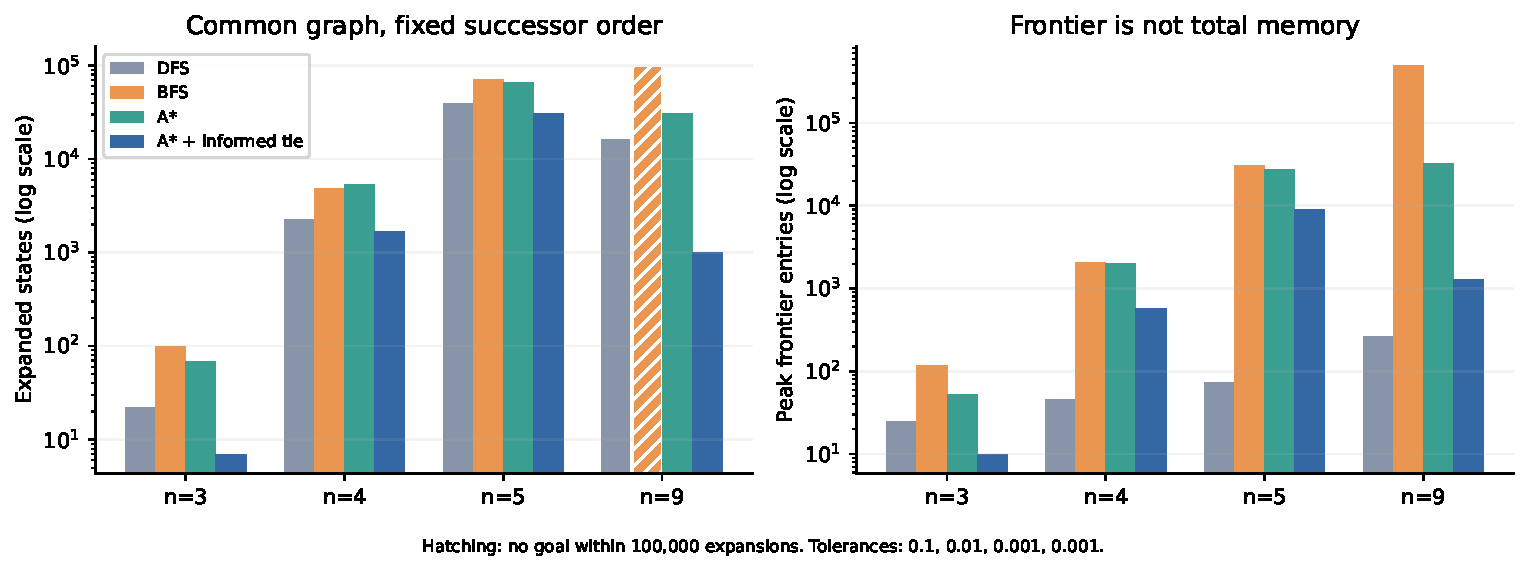
\includegraphics[width=.96\textwidth]{04/results/search_comparison.pdf}
\caption{共通状態グラフに対する探索の実測。左は展開数、右はフロンティア最大登録数。斜線は予算10万展開での打切りであり、解の不存在を意味しない。DFSも重複判定用辞書を保持するため、フロンティアが小さくても総メモリが定数になるわけではない。}
\label{fig:q04search}
\end{figure*}

表\ref{tab:q04nodes}と図\ref{fig:q04search}より、素朴なA*が常にDFSやBFSより少ない展開数になるわけではない。
$n=4$ではA*の5,362展開に対し、BFSは4,881展開であった。
下界が正しくても弱い場合、同点の並びが結果に影響するためである。
一方、A*+では全4例で展開数が減少した。
特に9桁ではA*の30,360から990へ減り、約30.7倍の差となった。
ただし決定論的な4例の結果であり、一般の数列や任意の目標値に対する優越性は主張しない。

9桁の場合、DFSは17操作で$99/70$を発見し、A*とA*+は5操作で
\[
 \frac{1.234}{.56}-.789
 =\frac{4951}{3500}
\]
を得た。
後者の絶対誤差は$3.5786620\times10^{-4}$、前者は$7.2151913\times10^{-5}$である。
すなわち、最短の式と最も正確な式は一致しない。
9桁の実測時間はDFSが0.123秒、BFSが打切りまで5.773秒、A*が0.437秒、A*+が0.061秒であった。
時間はmacOS 15.5/arm64、Python 3.9.6での1回の観測値であり、反復測定した平均ではない。
BFSの最大フロンティアは495,949登録に達した。

\subsection{区間DPと逆算による高精度探索}
高精度を要求すると通常の列挙探索は膨大になる。
そこで数字列を$1234\mid56789$または$12345\mid6789$に分け、左右それぞれの全ての括弧付けを区間動的計画法で列挙した。
各区間の辞書は「有理数$\mapsto$最小の演算子数を持つ代表式」とする。
左右の値の全組合せを根で試す代わりに、目標から逆算した右側の値を二分探索する。
例えば根が除算なら$a/b\simeq\sqrt{2}$に対し$b\simeq a/\sqrt{2}$を探す。
他の三則も同様に扱い、近傍候補と端点を検証した。
最終結果の誤差はDecimal 60桁で再計算した。
二分探索の位置決定には倍精度数を用いるため、これは測定した候補からの高精度解であり、全構文の大域最適性を主張するものではない。

\begin{figure}[tb]
\centering
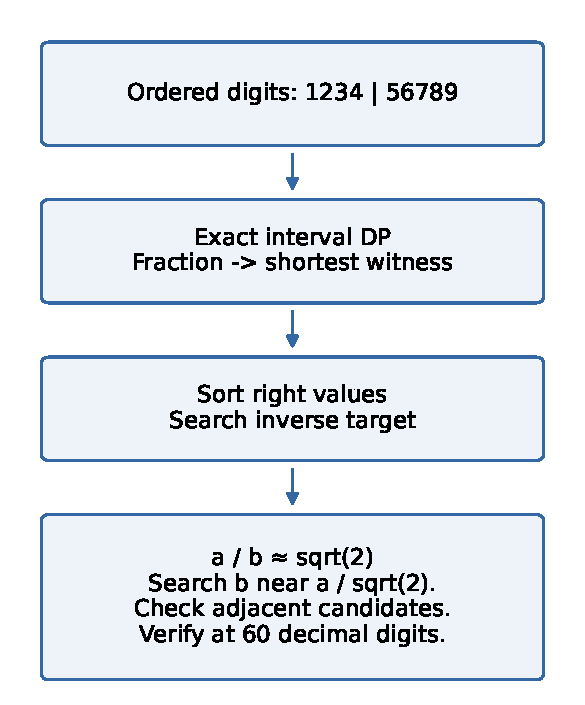
\includegraphics[width=\linewidth]{04/results/mitm_pipeline.pdf}
\caption{部分式を有理数の辞書に圧縮し、根の演算を逆算して組み合わせる。DFS/BFS/A*の実験にはこの前計算を使用していない。}
\label{fig:q04pipeline}
\end{figure}

$4\mid5$分割では、左に2,975、右に265,046種類の有理数が存在した。
根で単純に全組合せを作れば、四則それぞれについて約$7.9\times10^8$組を調べる必要がある。
逆算による候補照合は83,293回で済み、前計算込みの実測は約4秒であった。
順序固定で得られた式は
\begin{equation}
 \frac{(.1+2/.3)-.4}
 {\left(.5+\dfrac{6/.7}{8!}\right)9}
 =\frac{149744}{105885}.
 \label{eq:q04ordered}
\end{equation}
この値は$1.4142135335505501\ldots$、絶対誤差は
$2.8822545\times10^{-8}$である。
課題ページの順序固定例より約161倍小さい誤差となった。
各数字の使用順序は$1,2,3,4,5,6,7,8,9$であり、追加の数字定数を使用していない。

\subsection{数字を並べ替えた場合と「美しさ」}
固定した3つの並べ替え$987654321$、$371526498$、$824613975$について、同じ$4\mid5$分割を試した。
このうち$371526498$から
\begin{equation}
 \frac{3\{(.7+1)-5\}}
 {2-\dfrac{.6\times4!+9!}{8!}}
 \label{eq:q04permuted}
\end{equation}
を得た。絶対誤差は$1.8404692\times10^{-9}$であり、式\eqref{eq:q04ordered}より約15.7倍小さい。
ただし順列$9!$通りの網羅探索ではない。
並べ替えによって表現可能な分数が増え、良い近似に出会う機会は増すが、試したどの順列でも改善するわけではなかった。
課題ページの並べ替え例の誤差$9.2955\times10^{-12}$は、今回得た最良値よりさらに小さい。
したがって、今回の探索は既知例を上回る最高精度の達成を示すものではない。

\begin{figure*}[tb]
\centering
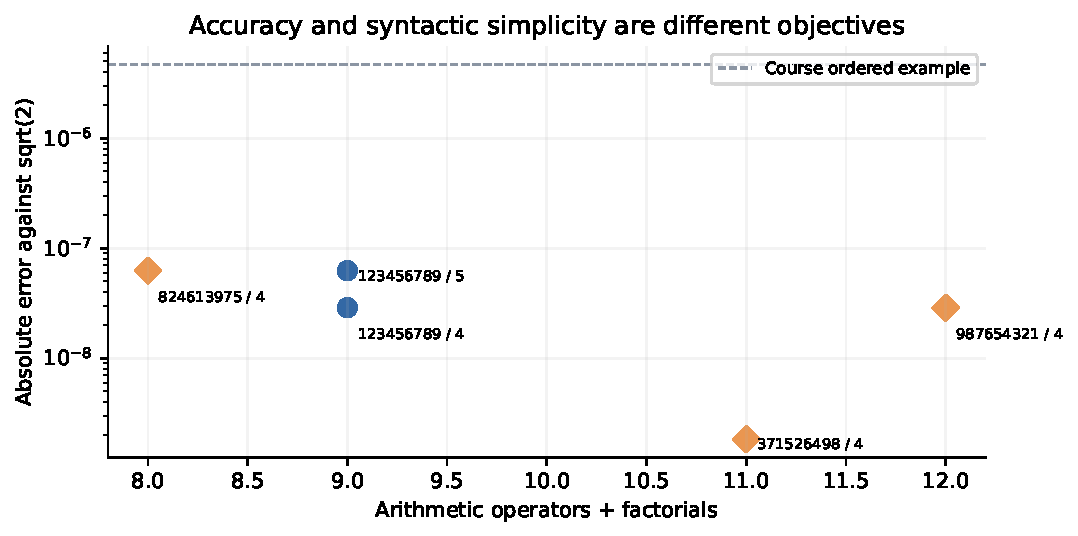
\includegraphics[width=.85\textwidth]{04/results/precision.pdf}
\caption{独立した高精度探索で得た式の精度と演算子数。丸は順序固定、菱形は並べ替え。図中の末尾の4または5は分割位置。階乗も演算子1個として数える。}
\label{fig:q04precision}
\end{figure*}

式の美しさは、精度とは別に、二項演算と階乗の合計個数、次いで括弧を含む文字数で評価した。
辞書内で同値の式を統合する際には、この順に短い表現を残した。
しかし最終候補はまず絶対誤差を優先して選んだため、図\ref{fig:q04precision}の各点は多目的最適化の完全なPareto前線ではない。
例えば、A*が得た2個の二項演算だけの式は読みやすい一方、式\eqref{eq:q04ordered}は9演算子、式\eqref{eq:q04permuted}は11演算子を要する。
用途に応じて許容誤差を先に決め、その範囲で最短の式を選ぶ方法が、近似と簡潔さを両立させやすい。

\subsection{実装上の工夫と残る課題}
実装では式と値を保持する不変データ型、四則演算、後継生成、探索方策、実験・描画を分離した。
数式文字列を実行する\texttt{eval}は使用しない。
単体テストでは小数・階乗の厳密値、ゼロ除算の排除、下界の整合性、小規模なRPN列挙と区間DPの到達値集合の一致、A*とBFSの最小操作数の一致を確認した。
元ページの近似値の誤植も有理数と60桁小数の両方で確認し、全パラメータと生結果を公開対象にした。

今後は全ての根の分割位置を扱う区間DP、式木の高さを加えた美しさの評価、より厳しい精度での探索法比較が考えられる。
現実装の下界は「あと何手か」という構造だけを見るため、値の到達可能性を表す区間や合同条件を許容的に組み込めれば、同点整列だけに依存しない削減が期待できる。
また、元の課題にある8パズルと異なり、全ての解の深さが同じとは限らないことを、連結を含む今回の文法で実際に確認できた。

\repolink{04}
